
\section{Modelo de datos}

Para plantear el modelo de datos,
adoptamos el enfoque de listar las diferentes tablas que puede necesitar cada uno de los actores.

El encargado de compras puede necesitar:
\begin{itemize}
	\item Precio de producto por proveedor 
	\item Productos por stock 
	\item Precio histórico por producto
\end{itemize}

El encargado de ventas puede necesitar:
\begin{itemize}
	\item Precio de producto por competidor
	\item Precio histórico de ventas por cliente
	\item Margen de ganancia por venta
\end{itemize}

El personal de ventas puede necesitar:
\begin{itemize}
	\item Precio por producto
	\item Productos por stock 
\end{itemize}

Las entidades serían entonces:
\begin{itemize}
	\item Producto
	\item Cliente 
	\item Proveedor 
	\item Competidor 
\end{itemize}

Las relaciones:
\begin{itemize}
	\item Producto-proveedor 
	\item Producto-cliente 
	\item Producto-competidor 
\end{itemize}

Dadas estas entidades y relaciones,
el modelo de datos entidad-relación propuesto se presenta a continuación:

\begin{figure}[ht]
	\centering
	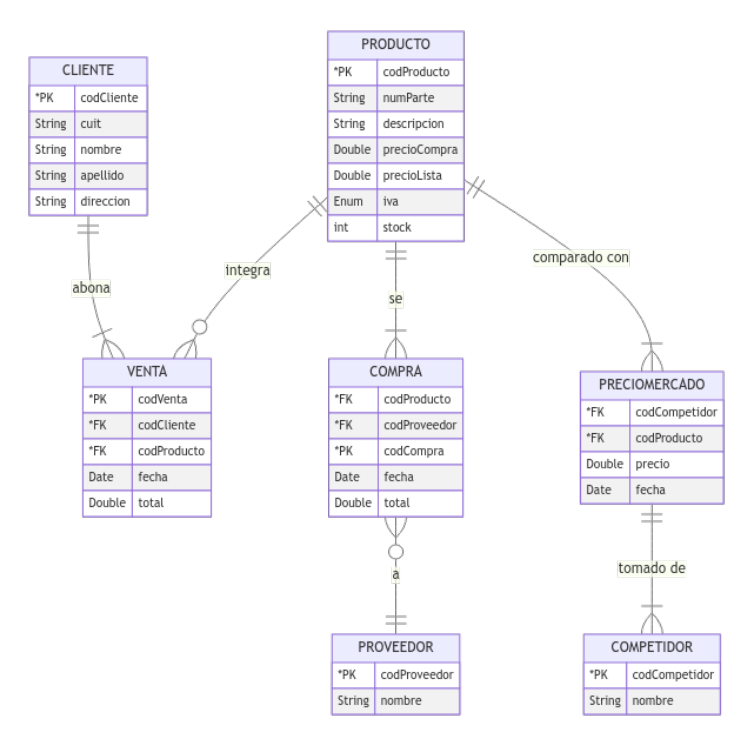
\includegraphics[width=\textwidth]{img/02-modelo-entidad-relacion}
	\caption{Modelo entidad-relación}
\end{figure}